\begin{center}
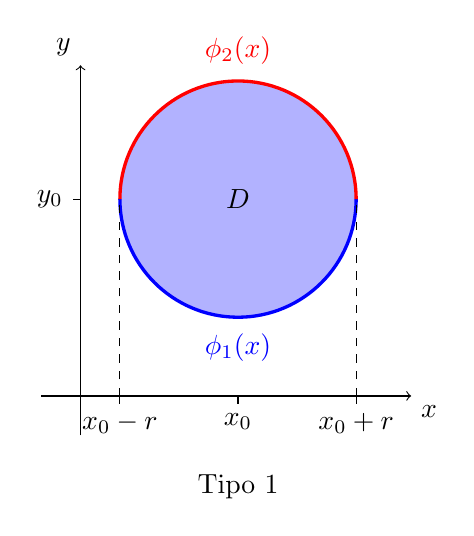
\begin{tikzpicture}
    % parámetros
    \def\cx{2}    % x_0
    \def\cy{2.5}    % y_0
    \def\rr{1.5}  % r

    %—————— Región Tipo 1 (despeje de y en función de x) ——————
    \begin{scope}
        % ejes
        \draw[->] (-0.5,0) -- (4.2,0) node[below right] {$x$};
        \draw[->] (0,-0.5) -- (0,4.2) node[above left]  {$y$};

        % relleno del círculo
        \fill[blue!30] (\cx,\cy) circle [radius=\rr];

        % semicircunferencia inferior: phi_1(x) = -sqrt(r-(x-x0)^2)+y0
        \draw[blue, very thick] (\cx-\rr,\cy) arc[start angle=180, end angle=360, radius=\rr]
            node[midway, below, yshift=-2pt] {\color{blue}$\phi_1(x)$};
        % semicircunferencia superior: phi_2(x) = +sqrt(r-(x-x0)^2)+y0
        \draw[red, very thick] (\cx-\rr,\cy) arc[start angle=180, end angle=0, radius=\rr]
            node[midway, above, yshift=2pt] {\color{red}$\phi_2(x)$};

        % líneas punteadas verticales en x_0 - r y x_0 + r
        \draw[dashed] (\cx-\rr,0) -- (\cx-\rr,\cy);
        \draw[dashed] (\cx+\rr,0) -- (\cx+\rr,\cy);

        % ticks y etiquetas en el eje x
        \draw (\cx-\rr,0) -- ++(0,-0.1) node[below] {$x_0-r$};
        \draw (\cx,0)     -- ++(0,-0.1) node[below] {$x_0$};
        \draw (\cx+\rr,0) -- ++(0,-0.1) node[below] {$x_0+r$};
        % tick y etiqueta en y_0
        \draw (0,\cy) -- ++(-0.1,0) node[left] {$y_0$};

        % etiqueta D
        \node at (\cx,\cy) {$D$};

        % título
        \node[below, yshift=-22pt] at (\cx,-0.1) {Tipo 1};
    \end{scope}
    \end{tikzpicture}
    \end{center}